LLVM IR is an alternative form of the program you want to optimize and compile. It is, however, structured differently from normal programming languages such as C/C++. LLVM IR is organized in a hierarchical fashion. The levels in this hierarchy – counting from the top – are Module, function, basic block, and instruction. The following diagram shows their structure:

\hspace*{\fill} \\ %插入空行
\begin{center}
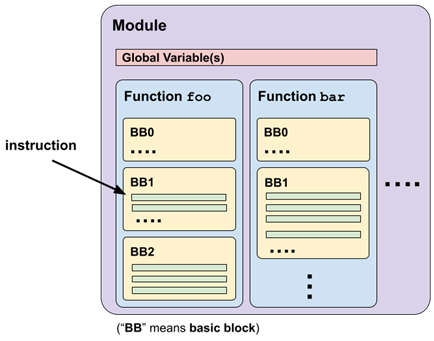
\includegraphics[width=0.9\textwidth]{content/3/chapter10/images/1.png}\\
Figure 10.1 – Hierarchy structure of LLVM IR
\end{center}

A module represents a translation unit – usually a source file. Each module can contain multiple functions (or global variables). Each contains a list of basic blocks where each of the basic blocks contains a list of instructions.

\begin{tcolorbox}[colback=blue!5!white,colframe=blue!75!black, fonttitle=\bfseries,title=Quick refresher – basic block]	
\hspace*{0.7cm}A basic block represents a list of instructions with only one entry and one exit point. In other words, if a basic block is executed, the control flow is guaranteed to walk through every instruction in the block.
\end{tcolorbox}

Knowing the high-level structure of LLVM IR, let's look at one of the LLVM IR examples. Let's say we have the following C code, foo.c:

\begin{lstlisting}[style=styleCXX]
int foo(int a, int b) {
	return a > 0? a – b : a + b;
}
\end{lstlisting}

We can use the following clang command to generate its textual LLVM IR counterpart:

\begin{tcblisting}{commandshell={}}
$ clang -emit-llvm -S foo.c
\end{tcblisting}

The result will be put in the foo.ll file. The following diagram shows part of its content, with annotations for the corresponding IR unit:

\hspace*{\fill} \\ %插入空行
\begin{center}
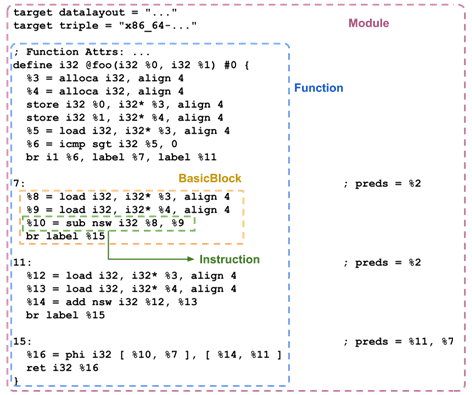
\includegraphics[width=0.9\textwidth]{content/3/chapter10/images/2.png}\\
Figure 10.2 – Part of the content in foo.ll, annotated with the corresponding IR unit
\end{center}

In textual form, an instruction is usually presented in the following format:

\begin{tcblisting}{commandshell={}}
<result> = <operator / op-code> <type>, [operand1, operand2, …]
\end{tcblisting}

For instance, let's assume we have the following instruction:

\begin{tcblisting}{commandshell={}}
%12 = load i32, i32* %3
\end{tcblisting}

Here, \%12 is the result value, load is the op-code, i32 is the data type of this instruction, and \%3 is the only operand.

In addition to the textual representation, nearly every component in LLVM IR has a C++ class counterpart with the same name. For instance, a function and a basic block are simply represented by Function and the BasicBlock C++ class, respectively.

Different kinds of instructions are represented by classes that are all derived from the Instruction class. For example, the BinaryOperator class represents a binary operation instruction, while ReturnInst class represents a return statement. We will look at Instruction and its child classes in more detail later.

The hierarchy depicted in Figure 10.1 is the concrete structure of LLVM IR. That is, this is how they are stored in memory. On top of that, LLVM also provides other logical structures to view the relationships of different IR units. They are usually evaluated from the concrete structures and stored as auxiliary data structures or treated as analysis results. Here are some of the most important ones in LLVM:

\begin{itemize}
\item Control Flow Graph (CFG): This is a graph structure that's organized into basic blocks to show their control flow relations. The vertices in this graph represent basic blocks, while the edges represent a single control flow transfer.

\item Loop: This represents the loop we are familiar with, which consists of multiple basic blocks that have at least one back edge – a control flow edge that goes back to its parent or ancestor vertices. We will look at this in more detail in the last section of this chapter, the Working with loops section.

\item Call graph: Similar to CFG, the call graph also shows control flow transfers, but the vertices become individual functions and the edges become function call relations.
\end{itemize}

In the next section, we are going to learn how to iterate through different IR units in both concrete and logical structures.

\subsubsubsection{10.2.1\hspace{0.2cm}Iterating different IR units}

Iterating IR units – such as basic blocks or instructions – are essential to LLVM IR development. It is usually one of the first steps we must complete in many transformation or analysis algorithms – scanning through the whole code and finding an interesting area in order to apply certain measurements. In this section, we are going to learn about the practical aspects of iterating different IR units. We will cover the following topics:

\begin{itemize}
\item Iterating instructions
\item Iterating basic blocks
\item Iterating the call graph
\item Learning the GraphTraits
\end{itemize}

Let's start by discussing how to iterate instructions.

\subsubsubsection{10.2.2\hspace{0.2cm}Iterating instructions}

An instruction is one of the most basic elements in LLVM IR. It usually represents a single action in the program, such as an arithmetic operation or a function call. Walking through all the instructions in a single basic block or function is the cornerstone of most program analyses and compiler optimizations.

To iterate through all the instructions in a basic block, you just need to use a simple for-each loop over the block:

\begin{lstlisting}[style=styleCXX]
// `BB` has the type of `BasicBlock&`
for (Instruction &I : BB) {
	// Work on `I`
}
\end{lstlisting}

We can iterate through all the instructions in a function in two ways. First, we can iterate over all the basic blocks in the function before visiting the instructions. Here is an example:

\begin{lstlisting}[style=styleCXX]
// `F` has the type of `Function&`
for (BasicBlock &BB : F) {
	for (Instruction &I : BB) {
		// Work on `I`
	}
}
\end{lstlisting}

Second, you can leverage a utility called inst\_iterator. Here is an example:

\begin{lstlisting}[style=styleCXX]
#include "llvm/IR/InstIterator.h"
…
// `F` has the type of `Function&`
for (Instruction &I : instructions(F)) {
	// Work on `I`
}
\end{lstlisting}

Using the preceding code, you can retrieve all the instructions in this function.

\hspace*{\fill} \\ %插入空行
\noindent
\textbf{Instruction visitor}

There are many cases where we want to apply different treatments to different types of instructions in a basic block or function. For example, let's assume we have the following code:

\begin{lstlisting}[style=styleCXX]
for (Instruction &I : instructions(F)) {
	switch (I.getOpcode()) {
		case Instruction::BinaryOperator:
		// this instruction is a binary operator like `add` or `sub`
		  break;
		case Instruction::Return:
		// this is a return instruction
		  break;
		…
	}
}
\end{lstlisting}

Recall that different kinds of instructions are modeled by (different) classes derived from Instruction. Therefore, an Instruction instance can represent any of them. The getOpcode method shown in the preceding snippet can give you a unique token – namely, Instruction::BinaryOperator and Instruction::Return in the given code – that tells you about the underlying class. However, if we want to work on the derived class ( ReturnInst, in this case) instance rather than the "raw" Instruction, we need to do some type casting.

LLVM provides a better way to implement this kind of visiting pattern –InstVisitor. InstVisitor is a class where each of its member methods is a callback function for a specific instruction type. You can define your own callbacks after inheriting from the InstVisitor class. For instance, check out the following code snippet:

\begin{lstlisting}[style=styleCXX]
#include "llvm/IR/InstVisitor.h"
class MyInstVisitor : public InstVisitor<MyInstVisitor> {
	void visitBinaryOperator(BinaryOperator &BOp) {
		// Work on binary operator instruction
		…
	}
	void visitReturnInst(ReturnInst &RI) {
		// Work on return instruction
		…
	}
};
\end{lstlisting}

Each visitXXX method shown here is a callback function for a specific instruction type. Note that we are not overriding each of these methods (there was no override keyword attached to the method). Also, instead of defining callbacks for all the instruction types, InstVisitor allows you to only define those that we are interested in.

Once MyInstVisitor has been defined, we can simply create an instance of it and invoke the visit method to launch the visiting process. Let's take the following code as an example:

\begin{lstlisting}[style=styleCXX]
// `F` has the type of `Function&`
MyInstVisitor Visitor;
Visitor.visit(F);
\end{lstlisting}

There are also visit methods for Instruction, BasicBlock, and Module.

\begin{tcolorbox}[colback=blue!5!white,colframe=blue!75!black, fonttitle=\bfseries,title=Ordering basic blocks and instructions]	
\hspace*{0.7cm}All the skills we've introduced in this section assume that the ordering of basic blocks or even instructions to visit is not your primary concern. However, it is important to know that Function doesn't store or iterate its enclosing BasicBlock instances in a particular linear order. We will show you how to iterate through all the basic blocks in various meaningful orders shortly.
\end{tcolorbox}

With that, you've learned several ways to iterate instructions from a basic block or a function. Now, let's learn how to iterate basic blocks in a function.

\subsubsubsection{10.2.3\hspace{0.2cm}Iterating basic blocks}

In the previous section, we learned how to iterate basic blocks of a function using a simple for loop. However, developers can only receive basic blocks in an arbitrary order in this way – that ordering gave you neither the execution order nor the control flow information among the blocks. In this section, we will show you how to iterate basic blocks in a more meaningful way.

Basic blocks are important elements for expressing the control flow of a function, which can be represented by a directed graph – namely, the CFG. To give you a concrete idea of what a typical CFG looks like, we can leverage one of the features in the opt tool. Assuming you have an LLVM IR file, foo.ll, you can use the following command to print out the CFG of each function in Graphviz format:

\begin{tcblisting}{commandshell={}}
$ opt -dot-cfg -disable-output foo.ll
\end{tcblisting}

This command will generate one .dot file for each function in foo.ll.

\begin{tcolorbox}[colback=blue!5!white,colframe=blue!75!black, fonttitle=\bfseries,title=The .dot File might be hidden]	
\hspace*{0.7cm}The filename of the CFG .dot file for each function usually starts with a dot character ('.'). On Linux/Unix systems, this effectively hides the file from the normal ls command. So, use the ls -a command to show those files instead.
\end{tcolorbox}

Each .dot file contains the Graphviz representation of that function's CFG. Graphviz is a general and textual format for expressing graphs. People usually convert a .dot file into other (image) formats before studying it. For instance, using the following command, you can convert a .dot file into a PNG image file that visually shows the graph:

\begin{tcblisting}{commandshell={}}
$ dot -Tpng foo.cfg.dot > foo.cfg.png
\end{tcblisting}

The following diagram shows two examples:

\hspace*{\fill} \\ %插入空行
\begin{center}
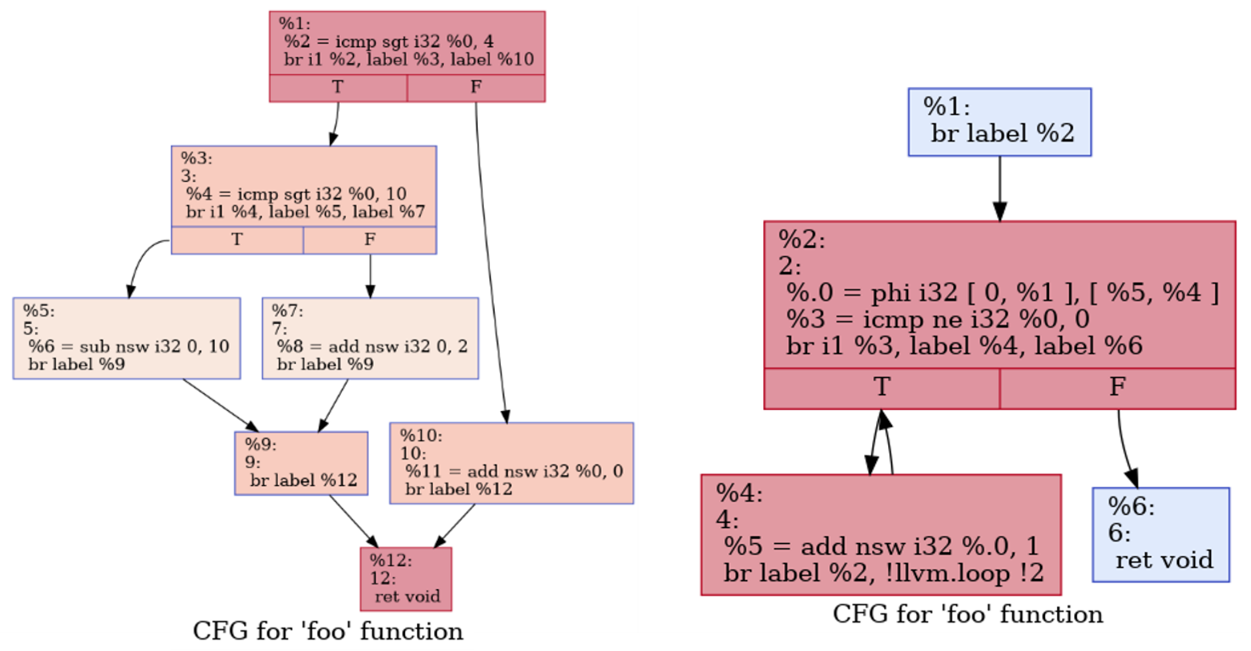
\includegraphics[width=0.9\textwidth]{content/3/chapter10/images/3.png}\\
Figure 10.3 – Left: CFG for a function containing branches; right: CFG for a function containing a loop
\end{center}

The left-hand side of the preceding diagram shows a CFG for a function containing several branches; the right-hand side shows a CFG for a function containing a single loop.

Now, we know that basic blocks are organized as a directed graph – namely, the CFG. Can we iterate this CFG so that it follows the edges and nodes? LLVM answers this question by providing utilities for iterating a graph in four different ways: topological order, depth first (essentially doing DFS), breadth first (essentially doing BFS), and Strongly Connected Components (SCCs). We are going to learn how to use each of these utilities in the following subsections.

Let's start with topological order traversal.

\hspace*{\fill} \\ %插入空行
\noindent
\textbf{Topological order traversal}

Topological ordering is a simple linear ordering that guarantees that for each node in the graph, it will only be visited after we've visited all of its parent (predecessor) nodes. LLVM provides po\_iterator and some other utility functions to implement reversed topological ordering (reversed topological ordering is easier to implement) on the CFG. The following snippet gives an example of using po\_iterator:

\begin{lstlisting}[style=styleCXX]
#include "llvm/ADT/PostOrderIterator.h"
#include "llvm/IR/CFG.h"
// `F` has the type of `Function*`
for (BasicBlock *BB : post_order(F)) {
	BB->printAsOperand(errs());
	errs() << "\n";
}
\end{lstlisting}

The post\_order function is just a helper function to create an iteration range of po\_iterator. Note that the llvm/IR/CFG.h header is necessary to make po\_iterator work on Function and BasicBlock.

If we apply the preceding code to the function containing branches in the preceding diagram, we'll get the following command-line output:

\begin{tcblisting}{commandshell={}}
label %12
label %9
label %5
label %7
label %3
label %10
label %1
\end{tcblisting}

Alternatively, you can traverse from a specific basic block using nearly the same syntax; for instance:

\begin{lstlisting}[style=styleCXX]
// `F` has the type of `Function*`
BasicBlock &EntryBB = F->getEntryBlock();
for (BasicBlock *BB : post_order(&EntryBB)) {
	BB->printAsOperand(errs());
	errs() << "\n";
}
\end{lstlisting}

The preceding snippet will give you the same result as the previous one since it's traveling from the entry block. You're free to traverse from the arbitrary block, though.

\hspace*{\fill} \\ %插入空行
\noindent
\textbf{Depth-first and breadth-first traversal}

DFS and BFS are two of the most famous and iconic algorithms for visiting topological structures such as a graph or a tree. For each node in a tree or a graph, DFS will always try to visit its child nodes before visiting other nodes that share the same parents (that is, the sibling nodes). On the other hand, BFS will traverse all the sibling nodes before moving to its child nodes.

LLVM provides df\_iterator and bf\_iterator (and some other utility functions) to implement depth-first and breadth-first ordering, respectively. Since their usages are nearly identical, we are only going to demonstrate df\_iterator here:

\begin{lstlisting}[style=styleCXX]
#include "llvm/ADT/DepthFirstIterator.h"
#include "llvm/IR/CFG.h"
// `F` has the type of `Function*`
for (BasicBlock *BB : depth_first(F)) {
	BB->printAsOperand(errs());
	errs() << "\n";
}
\end{lstlisting}

Similar to po\_iterator and post\_order, depth\_first is just a utility function for creating an iteration range of df\_iterator. To use bf\_iterator, simply replace depth\_first with breadth\_first. If you apply the preceding code to the containing branches in the preceding diagram, it will give you the following command-line output:

\begin{tcblisting}{commandshell={}}
label %1
label %3
label %5
label %9
label %12
label %7
label %10
\end{tcblisting}

When using bf\_iterator/breadth\_first, we will get the following command-line output for the same example:

\begin{tcblisting}{commandshell={}}
label %1
label %3
label %10
label %5
label %7
label %12
label %9
\end{tcblisting}

df\_iterator and bf\_iterator can also be used with BasicBlock, in the same way as po\_iterator shown previously.

\hspace*{\fill} \\ %插入空行
\noindent
\textbf{SSC traversal}

An SCC represents a subgraph where every enclosing node can be reached from every other node. In the context of CFG, it is useful to traverse CFG with loops.

The basic block traversal methods we introduced earlier are useful tools to reason about the control flow in a function. For a loop-free function, these methods give you a linear view that closely reflects the execution orders of enclosing basic blocks. However, for a function that contains loops, these (linear) traversal methods cannot show the cyclic execution flow that's created by the loops.

\begin{tcolorbox}[colback=blue!5!white,colframe=blue!75!black, fonttitle=\bfseries,title=Recurring control flow]	
\hspace*{0.7cm}Loops are not the only programming constructs that create recurring control flows within a function. A few other directives – the goto syntax in C/C++, for example – will also introduce a recurring control flow. However, those corner cases will make analyzing the control flow more difficult (which is one of the reasons you shouldn't use goto in your code), so when we are talking about recurring control flows, we are only referring to loops.
\end{tcolorbox}

Using scc\_iterator in LLVM, we can traverse strongly connected basic blocks in a CFG. With this information, we can quickly spot a recurring control flow, which is crucial for some analysis and program transformation tasks. For example, we need to know the back edges and recurring basic blocks in order to accurately propagate the branch probability data along the control flow edges.

Here is an example of using scc\_iterator:

\begin{lstlisting}[style=styleCXX]
#include "llvm/ADT/SCCIterator.h"
#include "llvm/IR/CFG.h"
// `F` has the type of `Function*`
for (auto SCCI = scc_begin(&F); !SCCI.isAtEnd(); ++SCCI) {
	const std::vector<BasicBlock*> &SCC = *SCCI;
	for (auto *BB : SCC) {
		BB->printAsOperand(errs());
		errs() << "\n";
	}
	errs() << "====\n";
}
\end{lstlisting}

Different from the previous traversal methods, scc\_iterator doesn't provide a handy range-style iteration. Instead, you need to create a scc\_iterator instance using scc\_begin and do manual increments. More importantly, you should use the isAtEnd method to check the exit condition, rather than doing a comparison with the "end" iterator like we usually do with C++ STL containers. A vector of BasicBlock can be dereferenced from a single scc\_iterator. These BasicBlock instances are the basic blocks within a SCC. The ordering among these SCC instances is roughly the same as in the reversed topological order – namely, the post ordering we saw earlier. 

If you run the preceding code over the function that contains a loop in the preceding diagram, it gives you the following command-line output:

\begin{tcblisting}{commandshell={}}
label %6
====
label %4
label %2
====
label %1
====
\end{tcblisting}

This shows that basic blocks \%4 and \%2 are in the same SCC. With that, you've learned how to iterate basic blocks within a function in different ways.

In the next section, we are going to learn how to iterate functions within a module by following the call graph.

\subsubsubsection{10.2.4\hspace{0.2cm}Iterating the call graph}

A call graph is a direct graph that represents the function call relationships in a module. It plays an important role in inter-procedural code transformation and analysis, namely, analyzing or optimizing code across multiple functions. A famous optimization called function inlining is an example of this.

Before we dive into the details of iterating nodes in the call graph, let's take a look at how to build a call graph. LLVM uses the CallGraph class to represent the call graph of a single Module. The following sample code uses a pass module to build a CallGraph:

\begin{lstlisting}[style=styleCXX]
#include "llvm/Analysis/CallGraph.h"
struct SimpleIPO : public PassInfoMixin<SimpleIPO> {
	PreservedAnalyses run(Module &M, ModuleAnalysisManager &MAM)
	{
		CallGraph CG(M);
		for (auto &Node : CG) {
			// Print function name
			if (Node.first)
			errs() << Node.first->getName() << "\n";
		}
		return PreservedAnalysis::all();
	}
};
\end{lstlisting}

This snippet built a CallGraph instance before iterating through all the enclosing functions and printing their names.

Just like Module and Function, CallGraph only provides the most basic way to enumerate all its enclosing components. So, how do we traverse CallGraph in different ways – for instance, by using SCC – as we saw in the previous section? The answer to this is surprisingly simple: in the exact same way – using the same set of APIs and the same usages.

The secret behind this is a thing called GraphTraits.

\subsubsubsection{10.2.5\hspace{0.2cm}Learning about GraphTraits}

GraphTraits is a class designed to provide an abstract interface over various different graphs in LLVM – CFG and call graph, to name a few. It allows other LLVM components – analyses, transformations, or iterator utilities, as we saw in the previous section – to build their works independently of the underlying graphs. Instead of asking every graph in LLVM to inherit from GraphTraits and implement the required functions, GraphTraits takes quite a different approach by using template specialization.

Let's say that you have written a simple C++ class that has a template argument that accepts arbitrary types, as shown here:

\begin{lstlisting}[style=styleCXX]
template <typename T>
struct Distance {
	static T compute(T &PointA, T &PointB) {
		return PointA – PointB;
	}
};
\end{lstlisting}

This C++ class will compute the distance between two points upon calling the Distance::compute method. The types of those points are parameterized by the T template argument.

If T is a numeric type such as int or float, everything will be fine. However, if T is a struct of a class, like the one here, then the default compute method implementation will not be able to compile:

\begin{lstlisting}[style=styleCXX]
Distance<int>::compute(94, 87); // Success
…
struct SimplePoint {
	float X, Y;
};
SimplePoint A, B;
Distance<SimplePoint>::compute(A, B); // Compilation Error
\end{lstlisting}

To solve this issue, you can either implement a subtract operator for SimplePoint, or you can use template specialization, as shown here:

\begin{lstlisting}[style=styleCXX]
// After the original declaration of struct Distance…
template<>
struct Distance<SimplePoint> {
	SimplePoint compute(SimplePoint &A, SimplePoint &B) {
		return std::sqrt(std::pow(A.X – B.X, 2),…);
	}
};
…
SimplePoint A, B;
Distance<SimplePoint>::compute(A, B); // Success
\end{lstlisting}

Distance<SimplePoint> in the previous code describes what Distance<T> looks like when T is equal to SimplePoint. You can think of the original Distance<T> as some kind of interface and Distance<SimplePoint> being one of its implementations. But be aware that the compute method in  Distance<SimplePoint> is not an override method of the original compute in Distance<T>. This is different from normal class inheritance (and virtual methods). 

GraphTraits in LLVM is a template class that provides an interface for various graph algorithms, such as df\_iterator and scc\_iterator, as we saw previously. Every graph in LLVM will implement this interface via template specialization. For instance, the following GraphTraits specialization is used for modeling the CFG of a function:

\begin{lstlisting}[style=styleCXX]
template<>
struct GraphTraits<Function*> {…}
\end{lstlisting}

Inside the body of GraphTraits<Function*>, there are several (static) methods and typedef statements that implement the required interface. For example, nodes\_iterator is the type that's used for iterating over all the vertices in CFG, while nodes\_begin provides you with the entry/starting node of this CFG:

\begin{lstlisting}[style=styleCXX]
template<>
struct GraphTraits<Function*> {
	typedef pointer_iterator<Function::iterator> nodes_iterator;
	static node_iterator nodes_begin(Function *F) {
		return nodes_iterator(F->begin());
	}
	…
};
\end{lstlisting}

In this case, nodes\_iterator is basically Function::iterator. nodes\_begin simply returns the first basic block in the function (via an iterator). If we look at GraphTraits for CallGraph, it has completely different implementations of nodes\_iterator and nodes\_begin:

\begin{lstlisting}[style=styleCXX]
template<>
struct GraphTraits<CallGraph*> {
	typedef mapped_iterator<CallGraph::iterator,
	decltype(&CGGetValuePtr)> nodes_iterator;
	static node_iterator nodes_begin(CallGraph *CG) {
		return nodes_iterator(CG->begin(), &CGGetValuePtr);
	}
};
\end{lstlisting}

When developers are implementing a new graph algorithm, instead of hardcoding it for each kind of graph in LLVM, they can build their algorithms by using GraphTraits as an interface to access the key properties of arbitrary graphs.

For example, let's say we want to create a new graph algorithm, find\_tail, which finds the first node in the graph that has no child nodes. Here is the skeleton of find\_tail:

\begin{lstlisting}[style=styleCXX]
template<class GraphTy,
typename GT = GraphTraits<GraphTy>>
auto find_tail(GraphTy G) {
	for(auto NI = GT::nodes_begin(G); NI != GT::nodes_end(G);
	++NI) {
		// A node in this graph
		auto Node = *NI;
		// Child iterator for this particular node
		auto ChildIt = GT::child_begin(Node);
		auto ChildItEnd = GT::child_end(Node);
		if (ChildIt == ChildItEnd)
		  // No child nodes
		  return Node;
	}
	…
}
\end{lstlisting}

With the help of this template and GraphTraits, we can reuse this function on Function, CallGraph, or any kind of graph in LLVM; for instance:

\begin{lstlisting}[style=styleCXX]
// `F` has the type of `Function*`
BasicBlock *TailBB = find_tail(F);
// `CG` has the type of `CallGraph*`
CallGraphNode *TailCGN = find_tail(CG);
\end{lstlisting}

In short, GraphTraits generalizes algorithms – such as df\_iterator and scc\_iterator, as we saw previously – in LLVM to arbitrary graphs using the template specialization technique. This is a clean and efficient way to define interfaces for reusable components.

In this section, we learned the hierarchy structure of LLVM IR and how to iterate different IR units – either concrete or logical units, such as CFGs. We also learned the important role of GraphTraits for encapsulating different graphs – CFGs and call graphs, to name a few – and exposed a common interface to various algorithms in LLVM, thus making those algorithms more concise and reusable.

In the next section, we will learn about how values are represented in LLVM, which describes a picture of how different LLVM IR components are associated with each other. In addition, we will learn about the correct and efficient way to manipulate and update values in LLVM.











